\documentclass[11pt,a4paper]{article}

\usepackage[utf8]{inputenc}
\usepackage[T1]{fontenc}
\usepackage[spanish,es-tabla]{babel}
\usepackage[margin=2.35cm]{geometry}
\usepackage{amsmath}
\usepackage{amssymb}
\usepackage{graphicx}
\usepackage{booktabs}
\usepackage{array}
\usepackage{float}
\usepackage{xcolor}
\usepackage{colortbl}
\definecolor{bestrow}{RGB}{220,245,220}
\definecolor{altrow}{RGB}{235,243,255}
\usepackage{microtype}
\usepackage{hyperref}
\usepackage{listings}
\usepackage{enumitem}
\usepackage{caption}

\microtypesetup{expansion=false}

\hypersetup{
    colorlinks=true,
    linkcolor=blue!60!black,
    citecolor=blue!60!black,
    urlcolor=blue!60!black
}

\lstdefinestyle{codestyle}{
    basicstyle=\ttfamily\small,
    breaklines=true,
    frame=single,
    columns=fullflexible,
    keepspaces=true,
    showstringspaces=false,
    tabsize=2,
    backgroundcolor=\color{gray!5}
}

\lstset{style=codestyle}

\graphicspath{{artifacts/figures/}}

\setlist[itemize]{leftmargin=1.2em}
\setlist[enumerate]{leftmargin=1.4em}

\title{\textbf{Predicción de fallos APS en camiones Scania}\\
\large Mantenimiento predictivo con datos tabulares, coste asimétrico, explicabilidad y robustez}

\author{
    Mauro Valls Vidal\\
    Alejandro Parra Sánchez\\
    Jordi Blasco Lozano\\
    Alejandro Martínez Riquelme\\[0.4em]
    \small Grado en Ingeniería en Inteligencia Artificial\\
    \small Escuela Politécnica Superior, Universidad de Alicante\\
    \small Aprendizaje Avanzado
}

\date{Curso 2025--2026}

\begin{document}

\maketitle

\begin{abstract}
Este trabajo presenta un estudio de aprendizaje automático para detectar fallos relacionados con el sistema APS de camiones Scania. La tarea se formula como clasificación binaria sobre datos tabulares industriales con 170 variables predictoras, valores faltantes, variables anonimizadas y una clase positiva muy minoritaria. El objetivo es identificar fallos APS y reducir el riesgo de falsos negativos. Los modelos se comparan mediante \texttt{Pipeline}, \texttt{GridSearchCV} y validación cruzada estratificada de 5 folds usando únicamente train. El mejor estimador se reentrena con todo train mediante \texttt{refit} y test queda reservado para la evaluación final. Se comparan un baseline, modelos lineales, SVM lineal, árboles y ensembles. El modelo principal seleccionado es \texttt{HistGradientBoosting}, con PR-AUC media de 0.881 en validación cruzada. En test obtiene PR-AUC de 0.922, F1 positivo de 0.842, recall positivo de 0.752, 13 falsos positivos y 93 falsos negativos. La memoria añade análisis de coste asimétrico, anomalías, importancia por permutación, robustez, errores y shift. La conclusión es que \texttt{HistGradientBoosting} es el modelo principal defendible, mientras que \texttt{logistic\_class\_weight} queda como alternativa operativa si se prioriza coste.
\end{abstract}

\noindent\textbf{Palabras clave}
Mantenimiento predictivo, Scania APS, clasificación binaria, datos tabulares, desbalanceo, PR-AUC, coste asimétrico, explicabilidad, robustez.

\tableofcontents
\newpage

\section{Introducción}
\label{sec_intro}

El mantenimiento predictivo busca anticipar fallos antes de que se conviertan en averías costosas. En vehículos industriales, una detección temprana puede reducir paradas, reparaciones innecesarias y riesgos operativos. Este proyecto se centra en el sistema APS de camiones Scania, relacionado con el suministro de aire a presión. Un fallo de este sistema puede afectar al funcionamiento del vehículo y generar costes importantes.

El problema tiene una dificultad práctica clara. Los fallos APS reales son poco frecuentes, por lo que la clase positiva aparece muy poco frente a la clase negativa. En este contexto, un modelo puede obtener una accuracy alta aunque ignore casi todos los fallos reales. Por esta razón, el proyecto no se evalúa solo con accuracy. Se usan métricas centradas en la clase positiva como recall, F1 y PR-AUC, junto con un coste asimétrico que penaliza más los falsos negativos.

La motivación del aprendizaje automático es aprovechar señales presentes en sensores, contadores y agregados internos del camión. Aunque las variables están anonimizadas, sus patrones estadísticos pueden ayudar a distinguir casos APS de casos no APS. La anonimización limita la interpretación física directa, pero no impide construir un modelo predictivo si el protocolo experimental se diseña con cuidado.

El objetivo del trabajo es construir y evaluar un flujo reproducible de aprendizaje automático para detectar fallos APS. El sistema no se presenta como una solución de producción. Es un estudio académico y técnico que compara modelos, analiza errores y discute limitaciones.

\section{Contribuciones del grupo}
\label{sec_contribuciones}

El trabajo desarrollado por el grupo se concreta en cuatro contribuciones principales. En primer lugar, se construye un flujo reproducible de preparación, exploración, modelado y auditoría para el dataset APS. En segundo lugar, se comparan modelos de familias distintas bajo un protocolo común con \texttt{Pipeline}, \texttt{GridSearchCV} y validación cruzada de 5 folds. En tercer lugar, se incorpora una lectura operativa del problema mediante coste asimétrico, análisis de falsos negativos y comparación de estrategias sensibles al desbalanceo. En cuarto lugar, se añaden análisis complementarios de anomalías, explicabilidad, robustez y shift que ayudan a interpretar el comportamiento del modelo más allá de una única métrica final.

La aportación no se limita a obtener un buen resultado en test. El objetivo ha sido construir una evaluación defendible, separando con claridad la selección realizada en train de la evaluación final realizada en test.

\subsection{Reparto de tareas}

El desarrollo se ha realizado de forma colaborativa, pero las responsabilidades principales se han distribuido de la siguiente manera:
\begin{itemize}
    \item \textbf{Mauro Valls Vidal}: Configuración general, exploración de datos (EDA), preprocesamiento e imputación.
    \item \textbf{Alejandro Parra Sanchez}: Implementación de los flujos de modelado supervisado, evaluación cruzada y selección de estimadores.
    \item \textbf{Jordi Blasco Lozano}: Análisis del impacto del desbalanceo, modelado de coste asimétrico y comparación de estrategias alternativas.
    \item \textbf{Alejandro Martínez Riquelme}: Implementación de las técnicas de auditoría (anomalías, importancia de variables, robustez al ruido, shift) y revisión final de la memoria.
\end{itemize}

\section{Contexto y trabajo relacionado}
\label{sec_contexto}

\subsection{Mantenimiento predictivo}

El mantenimiento predictivo aplica datos históricos y modelos estadísticos para anticipar fallos. Frente al mantenimiento correctivo, que actúa después de la avería, y al mantenimiento preventivo fijo, que programa revisiones por calendario, el mantenimiento predictivo intenta adaptar la intervención al estado observado del sistema.

En vehículos industriales, este enfoque es atractivo porque las averías pueden producir inmovilizaciones, retrasos y costes de reparación. Aun así, los modelos deben evaluarse con cautela. Un falso positivo puede generar una revisión innecesaria. Un falso negativo puede dejar pasar una avería real. En este proyecto, el falso negativo tiene un coste mucho mayor.

\subsection{Clasificación tabular y desbalanceo}

El dataset APS es tabular. Cada fila representa un caso de mantenimiento y cada columna describe una señal numérica. Este tipo de problema suele beneficiarse de árboles, bosques aleatorios y métodos de boosting, aunque los modelos lineales siguen siendo útiles como referencia.

El desbalanceo es una característica central. Si la clase positiva representa una proporción pequeña del total, la accuracy puede ser engañosa. Por eso se usan métricas que observan la clase positiva y el ranking de probabilidades. PR-AUC es especialmente relevante cuando los positivos son escasos, ya que resume la relación entre precisión y recall a distintos umbrales.

\subsection{Coste, explicabilidad y robustez}

En un problema industrial no todos los errores pesan igual. El dataset define un coste de 10 para falsos positivos y de 500 para falsos negativos. Este esquema no captura toda la complejidad real del mantenimiento, pero permite estudiar el impacto operativo de los errores.

La explicabilidad también importa. En este proyecto se usa importancia por permutación para estimar qué variables influyen más en el modelo. Esta técnica no demuestra causalidad. Sirve para auditar dependencias del modelo y detectar si el rendimiento depende de pocas variables.

La robustez se analiza añadiendo ruido a variables numéricas. Esta prueba no equivale a una validación de producción, pero ayuda a observar si pequeñas perturbaciones degradan mucho el rendimiento.

\section{Descripción del dataset}
\label{sec_dataset}

El dataset usado es \textit{APS Failure at Scania Trucks} del UCI Machine Learning Repository. Proporciona una partición oficial de entrenamiento y otra de test. La Tabla \ref{tab_dataset} resume sus características principales.

\begin{table}[H]
\centering
\caption{Características principales del dataset}
\label{tab_dataset}
\small
\begin{tabular}{@{}lr@{}}
\toprule
\textbf{Elemento} & \textbf{Valor}\\
\midrule
Train & 60000 filas\\
Test & 16000 filas\\
Variables predictoras & 170\\
Tipo de datos & Tabulares numéricos\\
Clase negativa original & \texttt{neg}\\
Clase positiva original & \texttt{pos}\\
Codificación usada & \texttt{neg} como 0 y \texttt{pos} como 1\\
Coste de falso positivo & 10\\
Coste de falso negativo & 500\\
\bottomrule
\end{tabular}
\end{table}

Las variables predictoras están anonimizadas. Proceden de sensores, contadores o agregados internos del camión, pero no se conoce su significado físico exacto. Esta anonimización es una limitación importante, porque dificulta interpretar por qué una variable concreta está asociada al fallo. Por ello, la memoria distingue entre importancia estadística e interpretación causal.

Los valores faltantes aparecen marcados como \texttt{na} en los archivos originales. En la preparación se convierten a valores faltantes reales. La variable objetivo se transforma a formato binario. La clase \texttt{pos} representa fallos relacionados con APS y es muy minoritaria. En train, la clase positiva representa alrededor del 1.67 por ciento de los casos.

\section{Análisis exploratorio}
\label{sec_eda}

\subsection{Distribución de clases y accuracy engañosa}

El primer resultado del EDA es el fuerte desbalanceo. La mayoría de observaciones pertenecen a la clase negativa. Un clasificador que predijera siempre la clase mayoritaria alcanzaría una accuracy muy alta, pero no detectaría fallos APS reales. Esta observación justifica que accuracy quede como métrica secundaria.

\begin{figure}[H]
\centering
\includegraphics[width=0.68\textwidth]{class_distribution_train.png}
\caption{Distribución de clases en train}
\label{fig_clases}
\end{figure}

La Figura \ref{fig_clases} muestra la desproporción entre negativos y positivos. Esta diferencia explica por qué el baseline puede parecer razonable si solo se mira accuracy, aunque sea incapaz de detectar la mayoría de fallos APS.

La evaluación se centra en recall positivo, F1 positivo, PR-AUC, balanced accuracy y coste. El recall positivo mide qué proporción de fallos APS se detecta. F1 positivo equilibra precisión y recall para la clase de interés. PR-AUC evalúa la calidad del ranking en un escenario con pocos positivos.

\subsection{Valores faltantes}

El dataset contiene muchos valores faltantes. Algunas variables presentan proporciones muy elevadas. En train, variables como \texttt{br\_000}, \texttt{bq\_000}, \texttt{bp\_000}, \texttt{bo\_000}, \texttt{ab\_000} y \texttt{cr\_000} superan el 77 por ciento de valores faltantes en varios casos. Esto hace que el tratamiento de missing values no sea un detalle menor.

\begin{figure}[H]
\centering
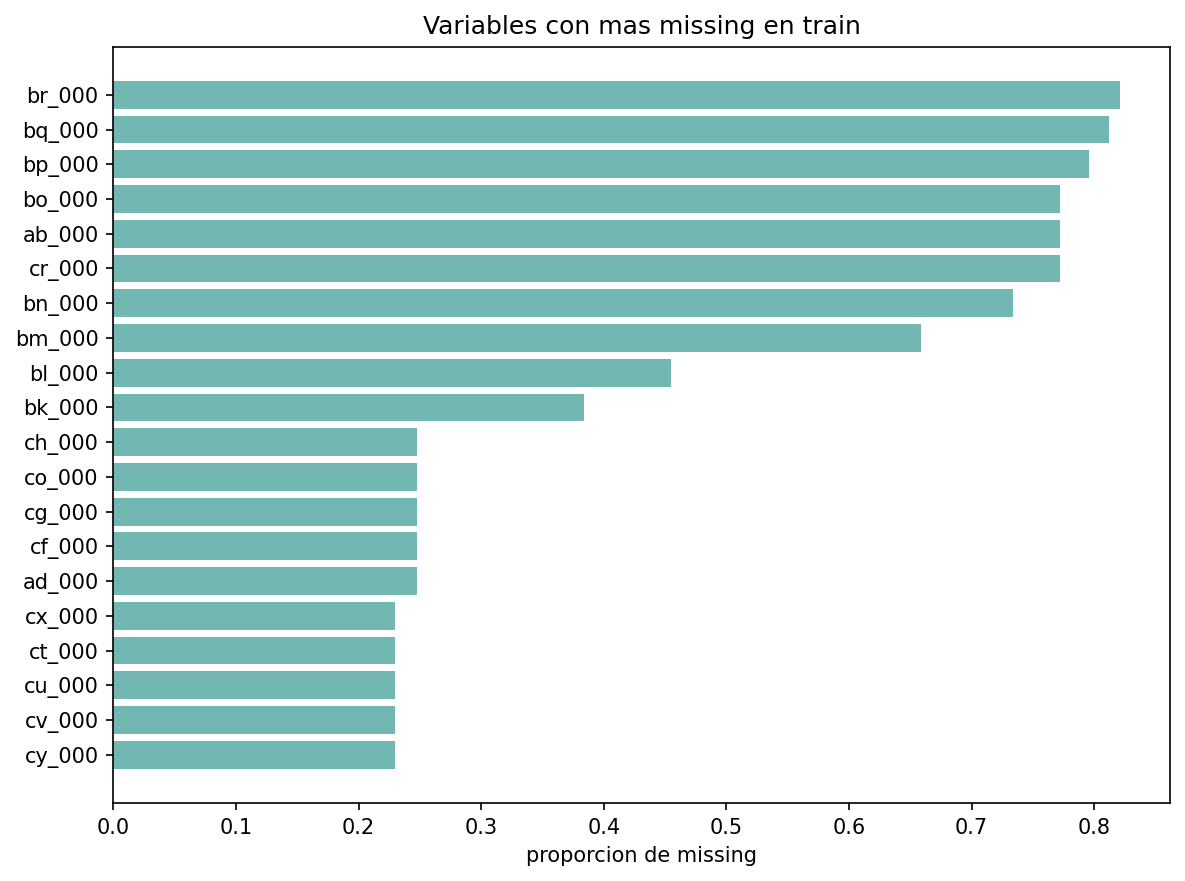
\includegraphics[width=0.82\textwidth]{missing_values_top30.png}
\caption{Variables con mayor proporción de valores faltantes en train}
\label{fig_missing}
\end{figure}

La Figura \ref{fig_missing} confirma que los missing values no aparecen de forma aislada. Hay grupos de variables con ausencia muy elevada, por lo que la imputación debe formar parte del procedimiento experimental y no ser un paso manual separado.

El EDA también compara el missing por clase. Algunas variables tienen patrones de ausencia muy distintos entre positivos y negativos. Por ejemplo, \texttt{ac\_000}, \texttt{ad\_000}, \texttt{ae\_000}, \texttt{af\_000} y \texttt{ak\_000} muestran más valores faltantes en la clase positiva. Otras variables, como \texttt{br\_000}, \texttt{bq\_000}, \texttt{bp\_000}, \texttt{bo\_000} y \texttt{bn\_000}, aparecen mucho más ausentes en la clase negativa.

La decisión metodológica derivada es no eliminar columnas manualmente desde el EDA. La imputación se introduce dentro de cada \texttt{Pipeline} mediante mediana. Así, en cada fold de validación cruzada, la mediana se calcula solo con la parte de entrenamiento correspondiente.

\subsection{Escalas, outliers y correlaciones}

Las variables tienen escalas muy diferentes. Algunas se concentran cerca de cero y otras alcanzan valores muy altos. También aparecen valores extremos. Según el análisis IQR, variables como \texttt{az\_007}, \texttt{dr\_000}, \texttt{dq\_000}, \texttt{bn\_000}, \texttt{ba\_008}, \texttt{cj\_000} y \texttt{aj\_000} tienen tasas elevadas de outliers.

Las correlaciones muestran redundancia entre algunas variables. Por ejemplo, \texttt{aa\_000} y \texttt{bt\_000} tienen una correlación prácticamente perfecta en la muestra analizada. También aparecen relaciones altas entre \texttt{ci\_000}, \texttt{ao\_000}, \texttt{bj\_000}, \texttt{bi\_000} y otras variables. Esta redundancia es habitual en datos de sensores.

Estas observaciones motivan el uso de escalado en modelos sensibles a escala, como regresión logística y SVM lineal. Los modelos basados en árboles no necesitan el mismo tratamiento, aunque todos mantienen imputación dentro del pipeline.

\section{Metodología}
\label{sec_metodologia}

\subsection{Protocolo experimental}

El protocolo experimental es una parte central del proyecto. La partición oficial de train se usa para explorar, entrenar y seleccionar modelos. La partición oficial de test se reserva para la evaluación final. El test no se usa para ajustar hiperparámetros, no ajusta umbrales, no elige modelo y no elige estrategia.

Los modelos se comparan con \texttt{GridSearchCV} y validación cruzada estratificada de 5 folds sobre train. El preprocesamiento forma parte de \texttt{Pipeline}, por lo que la imputación y el escalado se ajustan dentro de cada fold. Esto evita fuga de información desde validación hacia entrenamiento.

Después de la búsqueda, \texttt{GridSearchCV} reentrena el mejor estimador con todo train mediante \texttt{refit}. Solo entonces se evalúa en test. Las tablas de test se interpretan como comparación final o como auditoría posterior, nunca como criterio de selección.

\subsection{Modelos comparados}

La Tabla \ref{tab_modelos} resume los modelos supervisados comparados.

\begin{table}[H]
\centering
\caption{Modelos supervisados comparados}
\label{tab_modelos}
\small
\begin{tabular}{@{}lp{0.62\textwidth}@{}}
\toprule
\textbf{Familia} & \textbf{Modelos}\\
\midrule
Baseline & \texttt{DummyClassifier}\\
Modelos lineales & Regresión logística y SVM lineal\\
Árbol simple & Árbol de decisión\\
Ensembles & Random Forest, Extra Trees, AdaBoost e HistGradientBoosting\\
\bottomrule
\end{tabular}
\end{table}

Todos los modelos usan imputación con mediana. La regresión logística y la SVM lineal incorporan además \texttt{StandardScaler}. La métrica principal de selección es \texttt{average\_precision}, equivalente a PR-AUC. Como métricas complementarias se reportan recall positivo, F1 positivo, balanced accuracy, ROC-AUC y coste.

El coste se calcula con la expresión de la Ecuación \ref{eq_coste}.

\begin{equation}
\label{eq_coste}
C = 10 \cdot FP + 500 \cdot FN
\end{equation}

\section{Modelado supervisado}
\label{sec_modelado}

\subsection{Resultados de validación cruzada}

La Tabla \ref{tab_cv} muestra los resultados medios de validación cruzada sobre train. La tabla está ordenada por PR-AUC, que es la métrica principal de selección.

\begin{table}[H]
\centering
\caption{Comparativa de modelos con 5-fold CV sobre train}
\label{tab_cv}
\small
\begin{tabular}{@{}lrrrrr@{}}
\toprule
\textbf{Modelo} & \textbf{PR-AUC} & \textbf{Recall pos.} & \textbf{F1 pos.} & \textbf{Bal. acc.} & \textbf{Tiempo s}\\
\midrule
\rowcolor{bestrow} HistGradientBoosting & \textbf{0.881} & 0.738 & \textbf{0.809} & \textbf{0.868} & 35.9\\
Random Forest & 0.874 & 0.697 & 0.787 & 0.848 & 145.5\\
Extra Trees & 0.865 & 0.702 & 0.793 & 0.850 & 34.2\\
AdaBoost & 0.794 & 0.665 & 0.730 & 0.831 & 172.3\\
Logistic Regression & 0.772 & 0.632 & 0.708 & 0.815 & 31.3\\
Linear SVM & 0.769 & 0.619 & 0.708 & 0.808 & 1328.0\\
Decision Tree & 0.706 & 0.639 & 0.698 & 0.818 & 50.0\\
Dummy & 0.017 & 0.021 & 0.021 & 0.502 & 5.0\\
\bottomrule
\end{tabular}
\end{table}

El baseline confirma que una estrategia simple casi no detecta positivos. Los modelos avanzados mejoran de forma clara. \texttt{HistGradientBoosting} obtiene la mejor PR-AUC media con 0.881 y también el mejor F1 positivo. Random Forest y Extra Trees quedan cerca, pero no superan al modelo seleccionado en la métrica principal.

El tiempo de entrenamiento también es relevante. La SVM lineal tarda alrededor de 1328 segundos y no compensa esa duración porque queda por debajo de los ensembles principales. \texttt{HistGradientBoosting} ofrece un equilibrio favorable entre rendimiento y tiempo, ya que alcanza la mejor PR-AUC con un tiempo cercano al de Extra Trees y muy inferior al de Linear SVM y AdaBoost.

\subsection{Selección del modelo principal}

El modelo principal es \texttt{hist\_gradient\_boosting}. La selección se hace solo con validación cruzada en train y usando PR-AUC. El valor de selección guardado en los artefactos es 0.881018. Esta decisión se toma antes de analizar el rendimiento final en test.

\section{Resultados finales en test}
\label{sec_test}

Una vez seleccionado el modelo principal, se evalúa en test. La Tabla \ref{tab_test} muestra la comparativa final de los modelos ya ajustados.

\begin{table}[H]
\centering
\caption{Comparativa final en test}
\label{tab_test}
\small
\begin{tabular}{@{}lrrrrrr@{}}
\toprule
\textbf{Modelo} & \textbf{PR-AUC} & \textbf{Recall pos.} & \textbf{F1 pos.} & \textbf{FP} & \textbf{FN} & \textbf{Coste}\\
\midrule
\rowcolor{bestrow} HistGradientBoosting & \textbf{0.922} & \textbf{0.752} & \textbf{0.842} & \textbf{13} & \textbf{93} & \textbf{46630}\\
Random Forest & 0.920 & 0.717 & 0.816 & 15 & 106 & 53150\\
Extra Trees & 0.918 & 0.704 & 0.805 & 17 & 111 & 55670\\
AdaBoost & 0.840 & 0.680 & 0.753 & 47 & 120 & 60470\\
Logistic Regression & 0.819 & 0.701 & 0.767 & 48 & 112 & 56480\\
Linear SVM & 0.822 & 0.645 & 0.746 & 32 & 133 & 66820\\
Decision Tree & 0.770 & 0.645 & 0.748 & 30 & 133 & 66800\\
Dummy & 0.024 & 0.016 & 0.018 & 272 & 369 & 187220\\
\bottomrule
\end{tabular}
\end{table}

\texttt{HistGradientBoosting} mantiene un rendimiento fuerte en test. Obtiene PR-AUC de 0.922, F1 positivo de 0.842 y recall positivo de 0.752. La matriz de confusión se muestra en la Tabla \ref{tab_confusion}.

\begin{figure}[H]
\centering
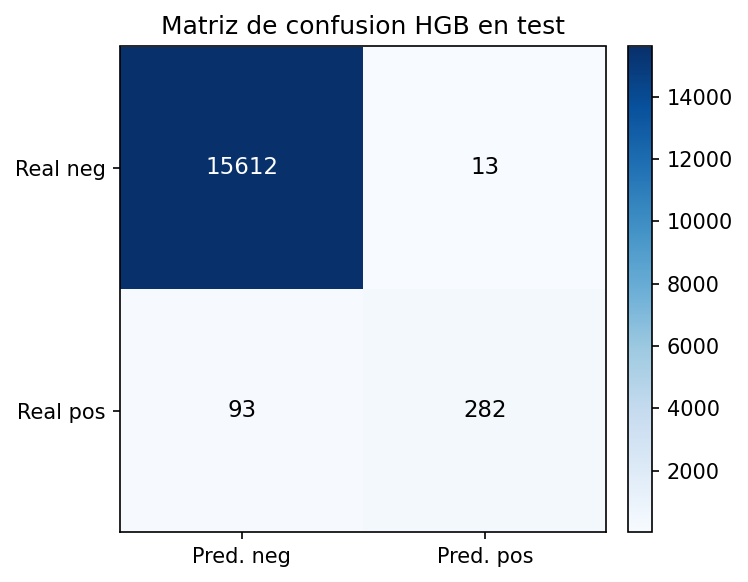
\includegraphics[width=0.58\textwidth]{confusion_matrix_best_model.png}
\caption{Matriz de confusión del modelo \texttt{HistGradientBoosting} en test}
\label{fig_confusion}
\end{figure}

La Figura \ref{fig_confusion} resume visualmente el comportamiento final. El bloque dominante corresponde a verdaderos negativos, pero el punto crítico está en la fila positiva. El modelo detecta 282 fallos APS y deja sin detectar 93.

\begin{table}[H]
\centering
\caption{Matriz de confusión del modelo principal en test}
\label{tab_confusion}
\small
\begin{tabular}{@{}lrr@{}}
\toprule
 & \textbf{Predicción negativa} & \textbf{Predicción positiva}\\
\midrule
Real negativo & 15612 & 13\\
Real positivo & 93 & 282\\
\bottomrule
\end{tabular}
\end{table}

La interpretación operativa es doble. El modelo genera pocas falsas alarmas, ya que solo produce 13 falsos positivos. Sin embargo, todavía deja pasar 93 fallos APS reales. Esto significa que el modelo es útil como sistema de apoyo, pero no es perfecto y no debe utilizarse sin supervisión.

\section{Desbalanceo y coste}
\label{sec_coste}

El notebook de desbalanceo y coste no sustituye al modelo principal. Su función es estudiar cómo cambian las métricas cuando se introducen estrategias sensibles al desbalanceo. Las estrategias comparadas son \texttt{hgb\_sin\_ajuste}, \texttt{logistic\_sin\_ajuste}, \texttt{logistic\_class\_weight} y \texttt{rf\_class\_weight}.

La selección por PR-AUC en validación cruzada vuelve a elegir \texttt{hgb\_sin\_ajuste}, con PR-AUC media de 0.881. La Tabla \ref{tab_coste} muestra la comparación final en test de estas estrategias.

\begin{table}[H]
\centering
\caption{Comparativa de estrategias de desbalanceo y coste en test}
\label{tab_coste}
\small
\begin{tabular}{@{}lrrrrrr@{}}
\toprule
\textbf{Estrategia} & \textbf{PR-AUC} & \textbf{Recall pos.} & \textbf{F1 pos.} & \textbf{FP} & \textbf{FN} & \textbf{Coste}\\
\midrule
\rowcolor{bestrow} \texttt{hgb\_sin\_ajuste} & 0.922 & 0.752 & \textbf{0.842} & \textbf{13} & 93 & 46630\\
\texttt{rf\_class\_weight} & 0.880 & 0.573 & 0.712 & 14 & 160 & 80140\\
\texttt{logistic\_sin\_ajuste} & 0.819 & 0.701 & 0.767 & 48 & 112 & 56480\\
\rowcolor{altrow} \texttt{logistic\_class\_weight} & 0.800 & \textbf{0.925} & 0.639 & 364 & \textbf{28} & \textbf{17640}\\
\bottomrule
\end{tabular}
\end{table}

\texttt{logistic\_class\_weight} reduce los falsos negativos de 93 a 28. A cambio aumenta los falsos positivos de 13 a 364 y reduce F1 positivo. Como el coste penaliza mucho más los falsos negativos, su coste total baja a 17640 frente a 46630 de \texttt{HistGradientBoosting}.

Este resultado no cambia el modelo principal. La razón es metodológica. El modelo principal se seleccionó por PR-AUC en train antes de mirar test. Si el objetivo principal fuese minimizar coste, habría que diseñar un experimento donde el coste se optimizara dentro de train mediante validación cruzada. No sería correcto escoger \texttt{logistic\_class\_weight} como modelo final solo porque su coste en test sea menor.

\section{Análisis de anomalías}
\label{sec_anomalias}

El análisis de anomalías es secundario. No sustituye al modelo supervisado. Su objetivo es comprobar si los fallos APS pueden detectarse como observaciones raras respecto a los casos normales.

Los detectores se entrenan con casos normales de train. Los umbrales se calculan usando train. Test se usa solo para evaluar. Se comparan Isolation Forest, Local Outlier Factor y One-Class SVM. La Tabla \ref{tab_anomalias} resume los resultados.

\begin{figure}[H]
\centering
\includegraphics[width=0.72\textwidth]{anomaly_scores_isolation_forest.png}
\caption{Distribución de scores de anomalía para Isolation Forest}
\label{fig_anomalias}
\end{figure}

La Figura \ref{fig_anomalias} ilustra la distribución de puntuaciones obtenidas por Isolation Forest, evidenciando la dificultad de separar ambas clases mediante un umbral estricto. Respecto a la comparativa global, la Tabla \ref{tab_anomalias} resume los resultados de los detectores en test.

\begin{table}[H]
\centering
\caption{Resultados de detección de anomalías en test}
\label{tab_anomalias}
\small
\begin{tabular}{@{}lrrrrrr@{}}
\toprule
\textbf{Detector} & \textbf{PR-AUC} & \textbf{Recall pos.} & \textbf{F1 pos.} & \textbf{FP} & \textbf{FN} & \textbf{Coste}\\
\midrule
Isolation Forest & 0.568 & 0.699 & 0.604 & 231 & 113 & 58810\\
Local Outlier Factor & 0.146 & 0.181 & 0.185 & 291 & 307 & 156410\\
One-Class SVM & \textbf{0.589} & \textbf{0.899} & 0.519 & 586 & \textbf{38} & \textbf{24860}\\
\bottomrule
\end{tabular}
\end{table}

One-Class SVM detecta muchos positivos y reduce los falsos negativos a 38. Sin embargo, genera 586 falsos positivos. Este comportamiento puede ser útil como sistema auxiliar de alerta si se acepta una carga alta de revisiones, pero no sustituye al modelo supervisado principal.

\section{Explicabilidad, robustez y errores}
\label{sec_xai}

\subsection{Importancia por permutación}

La importancia por permutación se calcula sobre una muestra de train y mide cuánto cae average precision cuando se desordena una variable. La Tabla \ref{tab_importancia} muestra las variables más influyentes.

\begin{figure}[H]
\centering
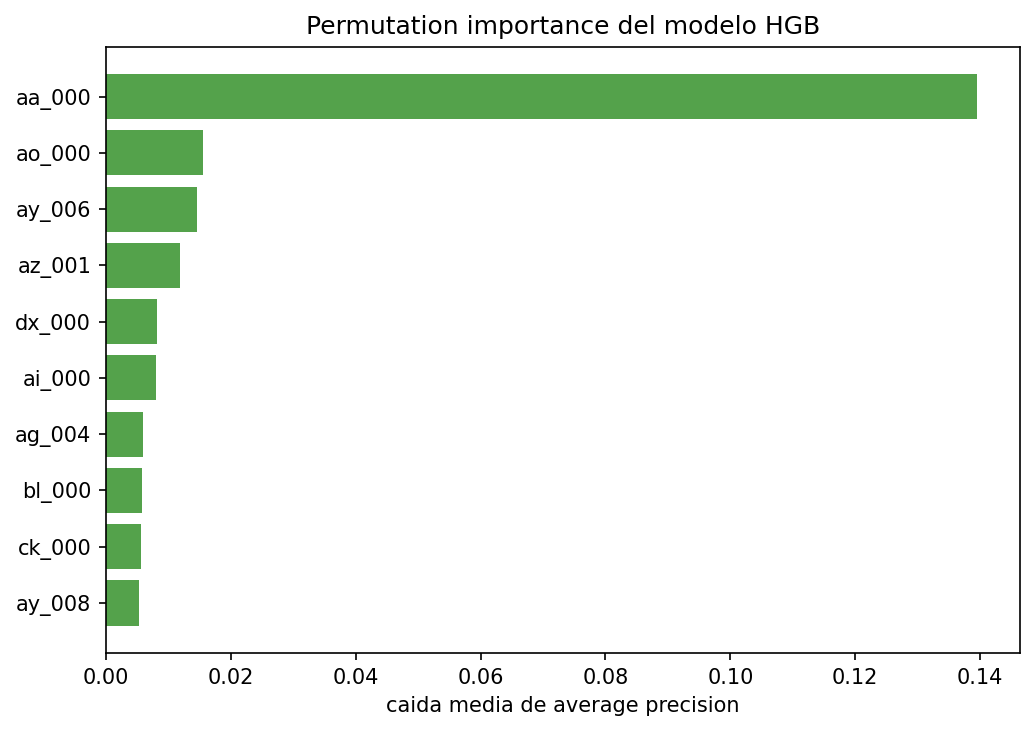
\includegraphics[width=0.78\textwidth]{feature_importance.png}
\caption{Importancia por permutación del modelo principal}
\label{fig_importancia}
\end{figure}

La Figura \ref{fig_importancia} permite ver que la importancia está muy concentrada. \texttt{aa\_000} destaca con mucha diferencia sobre el resto, lo que conviene tener en cuenta al interpretar la estabilidad del modelo.

\begin{table}[H]
\centering
\caption{Variables más importantes por permutation importance}
\label{tab_importancia}
\small
\begin{tabular}{@{}lrr@{}}
\toprule
\textbf{Variable} & \textbf{Importancia media} & \textbf{Desv.}\\
\midrule
\texttt{aa\_000} & 0.1394 & 0.0252\\
\texttt{ao\_000} & 0.0156 & 0.0013\\
\texttt{ay\_006} & 0.0145 & 0.0080\\
\texttt{az\_001} & 0.0118 & 0.0043\\
\texttt{dx\_000} & 0.0082 & 0.0041\\
\texttt{ai\_000} & 0.0080 & 0.0010\\
\texttt{ag\_004} & 0.0059 & 0.0063\\
\texttt{bl\_000} & 0.0059 & 0.0051\\
\texttt{ck\_000} & 0.0056 & 0.0006\\
\texttt{ay\_008} & 0.0054 & 0.0038\\
\bottomrule
\end{tabular}
\end{table}

\texttt{aa\_000} domina claramente el ranking. Al permutarla, la average precision cae alrededor de 0.139. La segunda variable, \texttt{ao\_000}, queda muy por debajo con una caída de 0.016. Esto sugiere que el modelo depende mucho de una señal principal. Debido a la anonimización, esta importancia no puede interpretarse como causa física del fallo.

\subsection{Análisis de errores}

El análisis de errores del modelo final muestra 15894 aciertos, 93 falsos negativos y 13 falsos positivos sobre 16000 observaciones de test. Un ejemplo local revisado en el notebook corresponde a un falso negativo. El caso real es positivo, pero el modelo lo predice como negativo. En ese ejemplo se inspeccionan los valores de las diez variables más importantes para entender el error desde las señales globales del modelo.

La principal limitación operativa sigue siendo el falso negativo. Aunque el número absoluto no es alto frente al tamaño total de test, cada falso negativo representa un fallo APS no detectado.

\subsection{Robustez ante ruido}

La prueba de robustez añade ruido a variables numéricas en una muestra de train. Es una auditoría de sensibilidad posterior al modelado, no una nueva evaluación final de test y no cambia la selección del modelo. La Tabla \ref{tab_robustez} resume la degradación observada.

\begin{figure}[H]
\centering
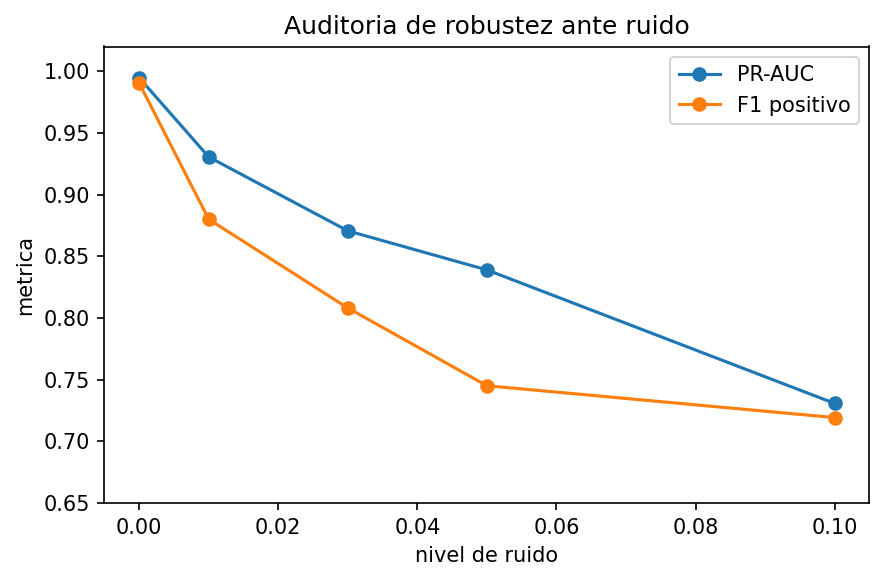
\includegraphics[width=0.72\textwidth]{robustness_curve.png}
\caption{Auditoría de sensibilidad ante ruido en variables numéricas}
\label{fig_robustez}
\end{figure}

La Figura \ref{fig_robustez} muestra una caída progresiva de PR-AUC y F1 positivo al aumentar el ruido. Esta lectura indica sensibilidad a perturbaciones en las señales, por lo que un uso real requeriría monitorizar la calidad de los datos de entrada.

\begin{table}[H]
\centering
\caption{Robustez ante ruido en variables numéricas}
\label{tab_robustez}
\small
\begin{tabular}{@{}rrrrrr@{}}
\toprule
\textbf{Ruido} & \textbf{PR-AUC} & \textbf{Recall pos.} & \textbf{F1 pos.} & \textbf{FP} & \textbf{FN}\\
\midrule
0.00 & 0.995 & 0.981 & 0.990 & 0 & 1\\
0.01 & 0.930 & 0.846 & 0.880 & 4 & 8\\
0.03 & 0.871 & 0.769 & 0.808 & 7 & 12\\
0.05 & 0.839 & 0.731 & 0.745 & 12 & 14\\
0.10 & 0.731 & 0.788 & 0.719 & 21 & 11\\
\bottomrule
\end{tabular}
\end{table}

El rendimiento cae al introducir perturbaciones. La caída de PR-AUC indica sensibilidad a la estabilidad de las señales numéricas. Esta prueba no invalida el modelo, pero muestra que un despliegue real debería monitorizar la calidad de los datos de entrada.

\subsection{Shift entre train y test}

El shift se analiza con el estadístico KS por variable entre train y test. Los valores más altos son bajos. \texttt{br\_000} alcanza 0.0227, \texttt{bq\_000} alcanza 0.0208, \texttt{ab\_000} alcanza 0.0152 y \texttt{bp\_000} alcanza 0.0145. El análisis no afirma deriva temporal, porque el dataset no representa un flujo ordenado en el tiempo. Solo indica que las distribuciones de train y test no parecen muy separadas en las variables revisadas.

\section{Discusión}
\label{sec_discusion}

\subsection{Por qué HistGradientBoosting es el modelo principal}

\texttt{HistGradientBoosting} es el modelo principal porque fue seleccionado por PR-AUC media en validación cruzada usando solo train. Además, mantiene el mejor rendimiento global en test entre los modelos comparados. Supera claramente al baseline, obtiene buen F1 positivo y genera muy pocos falsos positivos.

El resultado también es razonable desde el punto de vista técnico. Los modelos de boosting suelen funcionar bien en datos tabulares con relaciones no lineales e interacciones entre variables. En este proyecto, además, ofrece un buen equilibrio entre rendimiento y tiempo de entrenamiento.

\subsection{PR-AUC frente a coste}

PR-AUC y coste responden a preguntas distintas. PR-AUC evalúa la capacidad del modelo para ordenar positivos en un problema desbalanceado. El coste penaliza errores concretos con pesos distintos. Por eso \texttt{HistGradientBoosting} puede ser mejor por PR-AUC y \texttt{logistic\_class\_weight} puede ser mejor por coste en la comparativa final.

La conclusión correcta no es cambiar el modelo final mirando test. La lectura adecuada es que existe una alternativa operativa si el objetivo principal cambia. Para defender \texttt{logistic\_class\_weight} como modelo final habría que seleccionarlo dentro de train con una métrica de coste o con un protocolo de umbrales validado sin test.

\subsection{Limitaciones}

La primera limitación es la anonimización de variables. Se pueden detectar patrones estadísticos, pero no se puede explicar físicamente cada señal. La segunda limitación es el fuerte desbalanceo, que hace que pequeñas variaciones en falsos negativos tengan impacto relevante. La tercera limitación es el coste simplificado. La penalización de 10 y 500 es útil para comparar, pero no representa todos los costes reales de taller, logística y seguridad.

También hay limitaciones de evaluación. El proyecto usa una partición oficial de test, pero no valida el sistema en producción. No hay monitorización continua, validación temporal ni revisión por expertos de mantenimiento. Las pruebas de anomalías, robustez y shift son auditorías complementarias, no sustitutos de un despliegue real.

\subsection{Trabajo futuro}

Una mejora natural sería optimizar coste dentro de validación cruzada en train. Otra mejora sería estudiar umbrales de decisión con un conjunto de validación interno o validación cruzada, siempre sin usar test. También sería útil realizar validación temporal si se dispone de fechas, calibrar probabilidades y añadir revisión experta de falsos negativos.

En producción, sería necesario monitorizar drift, missing values, estabilidad de sensores, tasas de falsos negativos y coste real de intervención. También habría que diseñar una integración con procesos de mantenimiento y definir quién revisa las alertas.

\section{Conclusiones}
\label{sec_conclusiones}

El proyecto construye un flujo completo para detectar fallos APS en camiones Scania a partir de datos tabulares industriales. El dataset presenta dificultades reales como clase positiva minoritaria, valores faltantes, escalas diferentes, outliers, variables correlacionadas y anonimización.

El protocolo experimental cumple el criterio metodológico exigido. Los modelos se comparan con \texttt{GridSearchCV}, 5-fold CV y \texttt{Pipeline}. La selección de hiperparámetros se hace solo con train. El mejor estimador se reentrena con todo train mediante \texttt{refit}. Test se usa solo para evaluación final y auditoría posterior. No elige modelo, estrategia, umbral ni hiperparámetros.

El modelo principal es \texttt{HistGradientBoosting}. Se selecciona por PR-AUC en train, obtiene PR-AUC cercana a 0.881 en validación cruzada y mantiene PR-AUC cercana a 0.922 en test. En la evaluación final alcanza F1 positivo cercano a 0.842 y recall positivo cercano a 0.752. La matriz de confusión muestra 15612 verdaderos negativos, 282 verdaderos positivos, 13 falsos positivos y 93 falsos negativos.

El análisis de coste muestra que los falsos negativos siguen siendo importantes. \texttt{logistic\_class\_weight} reduce los falsos negativos a 28 y baja el coste total a 17640, pero aumenta mucho los falsos positivos y no fue el modelo seleccionado por la métrica principal en train. Por tanto, queda como alternativa operativa y no como modelo final.

Los análisis de anomalías, explicabilidad, robustez, errores y shift aportan una visión más completa. Las anomalías pueden servir como sistema auxiliar de alerta. La importancia por permutación muestra una dependencia fuerte de \texttt{aa\_000}. La robustez ante ruido evidencia sensibilidad a perturbaciones. El análisis de errores confirma que el modelo es útil, pero no perfecto.

En conjunto, el trabajo ofrece una solución técnica defendible para un problema real de mantenimiento predictivo. Su principal fortaleza no es solo el resultado de test, sino la separación estricta entre selección y evaluación, la comparación de modelos, la discusión de coste y la auditoría posterior del comportamiento.

\begin{table}[H]
\centering
\caption{Resumen final de conclusiones metodológicas}
\label{tab_conclusiones_metodologicas}
\small
\begin{tabular}{@{}p{0.32\textwidth}p{0.58\textwidth}@{}}
\toprule
\textbf{Aspecto} & \textbf{Conclusión}\\
\midrule
Modelo principal & \texttt{HistGradientBoosting}\\
Métrica de selección & PR-AUC media en 5-fold CV sobre train\\
Criterio metodológico & Cumplido mediante \texttt{Pipeline}, \texttt{GridSearchCV}, \texttt{refit} y test reservado solo para evaluación final\\
Mejor alternativa por coste & \texttt{logistic\_class\_weight}, con 28 falsos negativos y coste 17640 en test\\
Principal limitación & Variables anonimizadas, clase positiva minoritaria y coste simplificado\\
Trabajo futuro & Optimizar coste y umbrales dentro de train, validación temporal, calibración y revisión experta\\
\bottomrule
\end{tabular}
\end{table}

\section{Referencias}
\label{sec_referencias}

\begin{thebibliography}{9}

\bibitem{uciaps}
Dua, D. y Graff, C.
\newblock UCI Machine Learning Repository. APS Failure at Scania Trucks.
\newblock University of California, Irvine, School of Information and Computer Sciences.
\newblock \url{https://archive.ics.uci.edu/dataset/421/aps+failure+at+scania+trucks}

\bibitem{scikit}
Pedregosa, F. et al.
\newblock Scikit-learn. Machine Learning in Python.
\newblock \textit{Journal of Machine Learning Research}, 12, 2825--2830, 2011.

\bibitem{saito2015pr}
Saito, T. y Rehmsmeier, M.
\newblock The precision-recall plot is more informative than the ROC plot when evaluating binary classifiers on imbalanced datasets.
\newblock \textit{PLOS ONE}, 10(3), 2015.

\bibitem{fisher2019model}
Fisher, A., Rudin, C. y Dominici, F.
\newblock All models are wrong, but many are useful. Learning a variable's importance by studying an entire class of prediction models simultaneously.
\newblock \textit{Journal of Machine Learning Research}, 20(177), 1--81, 2019.

\bibitem{gama2014drift}
Gama, J., Zliobaite, I., Bifet, A., Pechenizkiy, M. y Bouchachia, A.
\newblock A survey on concept drift adaptation.
\newblock \textit{ACM Computing Surveys}, 46(4), 2014.

\end{thebibliography}

\appendix

\section{Anexo A. Archivos principales del flujo}
\label{anexo_archivos}

\begin{table}[H]
\centering
\caption{Archivos principales del flujo experimental}
\small
\begin{tabular}{@{}p{0.34\textwidth}p{0.56\textwidth}@{}}
\toprule
\textbf{Archivo} & \textbf{Uso en la memoria}\\
\midrule
\texttt{README.md} & Resumen del proyecto, protocolo, resultados y limitaciones.\\
\texttt{project\_utils.py} & Constantes de coste, funciones de carga, métricas, matriz de confusión y cálculo de coste.\\
\texttt{requirements.txt} & Dependencias y entorno de ejecución.\\
\texttt{00\_descarga\_y\_preparacion.ipynb} & Carga, limpieza inicial y codificación de clases.\\
\texttt{01\_EDA.ipynb} & Desbalanceo, missing values, outliers, correlaciones y métricas.\\
\texttt{02\_modelado\_supervisado.ipynb} & Modelos, \texttt{GridSearchCV}, CV, selección de HGB y resultados en test.\\
\texttt{03\_desbalanceo\_y\_coste.ipynb} & Estrategias de coste y comparación con \texttt{logistic\_class\_weight}.\\
\texttt{04\_anomalias.ipynb} & Detectores de anomalías y evaluación secundaria.\\
\texttt{05\_xai\_robustez\_errores.ipynb} & Importancia, errores, robustez y shift.\\
\bottomrule
\end{tabular}
\end{table}

El notebook \texttt{06\_resultados\_memoria\_y\_defensa.ipynb} se revisó solo como apoyo interno para contrastar tablas y mensajes de defensa. No se presenta como parte principal del flujo experimental entregable.

\section{Anexo B. Reproducción}
\label{anexo_reproduccion}

Para reproducir el proyecto se recomienda crear un entorno limpio e instalar las dependencias.

\begin{lstlisting}[language=bash]
python -m venv .venv
.venv\Scripts\activate
pip install -r requirements.txt
\end{lstlisting}

En Linux o macOS, la activación cambia a \texttt{source .venv/bin/activate}. También puede usarse un entorno conda equivalente instalando \texttt{requirements.txt}.

Después se ejecutan los notebooks desde la raíz del proyecto.

\begin{lstlisting}[language=bash]
jupyter nbconvert --to notebook --execute 00_descarga_y_preparacion.ipynb --inplace
jupyter nbconvert --to notebook --execute 01_EDA.ipynb --inplace
jupyter nbconvert --to notebook --execute 02_modelado_supervisado.ipynb --inplace
jupyter nbconvert --to notebook --execute 03_desbalanceo_y_coste.ipynb --inplace
jupyter nbconvert --to notebook --execute 04_anomalias.ipynb --inplace
jupyter nbconvert --to notebook --execute 05_xai_robustez_errores.ipynb --inplace
\end{lstlisting}

\end{document}
